\chapter{Analysis}

The analysis section of the thesis starts with demonstration of interactive
proofs with goal to build up intuition behind interactive proofs \cite{Goldwasser1989,youtubeMOOCLecture1}.
This section explains how Alice attempts to prove to Bob that she knows an
algorithm, with which she computes some pair (N, y), such that this pair is
part of the quadratic residue language QR. Specifically, Alice needs to
convince Bob that there exists an x such that y equals x squared modulo N,
effectively placing the pair (N, y) within the QR language, which includes all
pairs where y is a quadratic residue of N.

The analysis section continues by highlighting a practical limitation of
interactive proofs in real world cryptography. It notes that for Alice to
prove something to multiple parties, she would need to engage in separate
interactions with each one. This approach is not scalable and becomes
impractical for widespread verification needs. However, the thesis introduces
the Fiat-Shamir transform \cite{Fiat}, a significant breakthrough that addresses this
issue. This transform allows for converting the interactive proof into a
non-interactive format by processing the interaction transcript, making the
proof more practical and scalable for real-world cryptographic applications.

While in theory any NP statement \cite{Goldwasser1989} can be proven using
interactive proofs, practical implementation requires specific definition and
encoding of the statement. There are two main models of general computation,
those are circuits and turing machines. To trace the computation of a turing
machine, the representation needs to somehow handle memory and thus would accrue
more complexity than if a circuit is used. To represent a statement as a
circuit, an arithmetic circuit, a computation model composed of addition and
multiplication operations, is used. This circuit encodes the statement into a
form suitable for "zk-ifying", enabling the application of interactive proofs
to a broader range of practical scenarios.

The analysis section then explores various ZKP systems, each with unique
properties and proof constructions. The most renowned among these are SNARKs
(Succinct Non-interactive ARguments of Knowledge), Bulletproofs, and STARKs
(Scalable Transparent ARguments of Knowledge). These systems differ in aspects
such as computational efficiency, size of proofs, and the need (or lack
thereof) for a trusted setup. Each system offers advantages and challenges,
making them suitable for different applications.

The final part of the analysis examines how ZKP systems such as SNARKs enable
the creation of a stealth address scheme that upholds privacy and security.
This section assesses how these systems fulfill the necessary properties for a
stealth address scheme, focusing on their ability to ensure transaction
confidentiality while maintaining the anonymity of the recipient's identity.

\section{Proof of quadratic residuosity}

This first part focuses on demonstrating an interactive proof where Alice aims
to prove to Bob that she knows an algorithm, which computes some pair (N, y),
such that this pair is part of the quadratic residue language QR \cite{Goldwasser1989}.
QR is defined as:

\[QR = \lbrace(N, y): \exists x, y \equiv x^2 \pmod{N}\rbrace\]

\begin{figure}[h!]
    \centering
    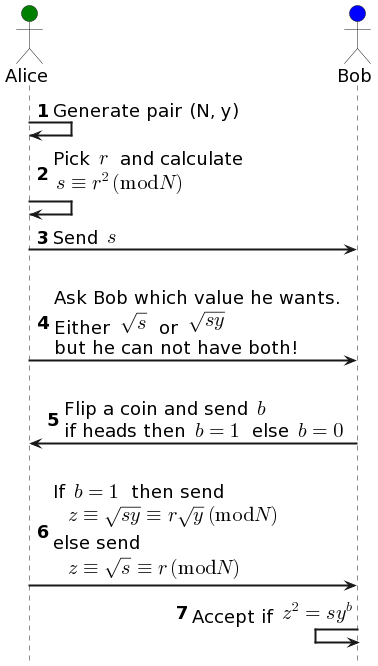
\includegraphics[scale=0.6]{assets/images/qr_ip.png}
    \caption{Interactive proof of language QR}
    \label{fig:qr_ip}
    \vspace{0.5cm}
\end{figure}

\begin{enumerate}
    \item Alice generates pair (N, y)
    \item Alice picks a random $r$ such that $1 \leq r \leq N$ and $\gcd(r, N) = 1$
          and calculates $s \equiv r^2 \pmod{N}$
    \item Alice sends Bob $s$
    \item Alice asks Bob which value he wants. Either $\sqrt{s}$ or $\sqrt{sy}$, but he can not have both!
    \item Bob flips a coin and sends $b$ such that if coin landed on heads $b = 1$ else $b = 0$
    \item If $b = 1$ Alice sends to Bob $z \equiv \sqrt{sy} \equiv r \sqrt{y} \pmod{N}$ else she sends $z \equiv \sqrt{s} \equiv r \pmod{N}$
    \item Bob accepts if $z^2 = sy^b$
\end{enumerate}

If Alice was a cheating prover, and she didn't have the algorithm for
generating pairs from QR, then the probability that Bob's coin toss favors
Alice is one half. With one half probability Bob would ask cheating prover
Alice to give him the equation she can not solve, because if the prover is
cheating, she can not find the $\sqrt{s}$ and $\sqrt{sy}$. If she could,
that would mean that she is not cheating.

If the Alice's claim is true, Bob will accept. If Alice is not honest, and
cheats, all provers will not accept with probability $P(Accept) = 0.5$.
But this probability may not be satisfying enough. To make the probability
that Alice is cheating smaller, Bob and Alice can start the interaction once
again. This would lead to $P(Accept) = (0.5)^2$. They can redo the process
as many times as they wish, resulting in $P(Accept) = (0.5)^k$ where $k$
is how many different interactions they performed.

Thanks to the randomness of the coin toss, there are $2^k$ possibilities how
the interaction can go. Since Alice can't reliably predict what the random
coin toss will yield, she must be ready to provide both equations. Thus Bob is
convinced, that Alice isn't cheating, with probability $P(Accept) = (0.5)^k$,
and can accept the proof.

\section{Arithmetic circuit}
in a finite field $\mathbb{F}_p$

% the interaction part is non-practical => Fiat Shamir

% R1Cs

% SNARKs - from Dan Boneh MOOC
% commitments
% SZDL lemma = a polynomial is zero-polynomial with d\/p probability = zero - test
